%%  By Himarsha R. Jayanetti and Dr. Michele C. Weigle
%%  April 16, 2024

%% The font size of the dissertation should be consistent at 12 pt
\documentclass[12pt]{report}

%%%%% Thesis or Dissertation Selection %%%%% 
%% For MS thesis, comment out the \usepackage{odusci} line (line 13) and 
%% uncomment the \usepackage[thesis]{odusci} line (line 17)

%% The default is for PhD dissertations
\usepackage{odusci}
%\usepackage[diss]{odusci}  % alternate PhD package specification
%% Uncomment this line for MS thesis
%\usepackage[thesis]{odusci}  

%%%%% Citation Style %%%%% 
%% Uncomment the appropriate line for your discipline
%% IEEE
\usepackage[style=ieee, sorting=nyt, maxnames=10, minnames=10]{biblatex}
%% APA
% \usepackage[style=apa, sorting=nyt, maxnames=10, minnames=10]{biblatex}
%% Science 
% \usepackage[style=science, sorting=nyt, maxnames=10, minnames=10]{biblatex}

%% add BibTeX file
\addbibresource{ref.bib}

%% ***DO NOT CHANGE OR COMMENT THE NEXT LINE*** 
\setlength\intextsep{1.69cm} % to set space above/below the floats and text 
\begin{document}

%%%%% TITLE PAGE %%%%% 
\title{THE TITLE OF THE DISSERTATION. PLEASE REPLACE THE TEXT HERE WITH YOUR TITLE}

\author{Jane Ann Doe}

%% US degree
\degrees{B.S. July 2017, Stanford University \\
         M.S. July 2020, Stanford University}

%% Use the following format if the prior degrees are outside of the US. 
%% University and Country must be all in a single line.
% \degrees{B.S. July 2017, University of Oxford, United Kingdom. \\
%          M.S. July 2020, University of Oxford,  United Kingdom.}

%% Department
\dept{Computer Science}

%% Generates Copyright page, do not uncomment for thesis or dissertation
%\copyrightfalse

%% submit date must use either "May", "August", or "December" for the month
\submitdate{May 2024}
% \submitdate{August 2024}
% \submitdate{December 2024}

%% Default is for a single adviser
\principaladviser{Director Name}
\member{Member Name}
\member{Member Name}
\member{Member Name}

%% Co-advisers - uncomment below if required
% \coadvisers{Director Name1}
% \coadvisers{Director Name2}
% \member{Member Name}
% \member{Member Name}
% \member{Member Name}
%% See https://github.com/oduwsdl/odusci-etd-template/blob/main/README.md
%% for instructions on adjusting odusci.sty to allow co-advisers

%%%%% FRONT MATTER %%%%% 

%% Abstract - maximum 350 words
\abstract{Lorem ipsum dolor sit amet, consectetur adipiscing elit. In non molestie odio. Pellentesque volutpat, sem a viverra dictum, leo est scelerisque risus, ut convallis dui nulla a lacus. Proin mi magna, pharetra non ante sit amet, euismod lobortis odio. Donec gravida eu elit quis sagittis. Duis consequat, elit in fermentum rutrum, tellus dolor sodales ante, ac aliquam libero purus eu nisi. In aliquam nibh maximus varius blandit. Sed consequat libero faucibus vehicula gravida. Suspendisse vitae nisi ex. Quisque gravida risus ac dapibus blandit. Vestibulum mollis sollicitudin justo. Donec vel ipsum non ligula efficitur consequat. Morbi vulputate feugiat diam, rhoncus vehicula eros posuere vitae. Pellentesque sed egestas metus. Vestibulum libero elit, euismod quis vestibulum nec, vulputate at risus. In accumsan sem eu porta ultrices. Quisque sagittis massa felis, eget varius metus semper id. Vivamus tincidunt ipsum sem, sit amet eleifend diam tempor nec. Vivamus elementum, diam id lobortis mattis, nisi lacus.} 

%% Dedication - optional, 1 page max
\dedication{I dedicate my dissertation ... Morbi vulputate feugiat diam, rhoncus vehicula eros posuere vitae. Pellentesque sed egestas metus.}

%% Acknowledgements
\acknowledge{I would like to thank...Lorem ipsum dolor sit amet, consectetur adipiscing elit. In non molestie odio. Pellentesque volutpat, sem a viverra dictum, leo est scelerisque risus, ut convallis dui nulla a lacus. Proin mi magna, pharetra non ante sit amet, euismod lobortis odio. Donec gravida eu elit quis sagittis. Duis consequat, elit in fermentum rutrum, tellus dolor sodales ante, ac aliquam libero purus eu nisi. In aliquam nibh maximus varius blandit. Sed consequat libero faucibus vehicula gravida. Suspendisse vitae nisi ex. Quisque gravida risus ac dapibus blandit. Vestibulum mollis sollicitudin justo. Donec vel ipsum non ligula efficitur consequat. 
%% If you want multiple paragraphs, must add a newline and indent as below
\\ \indent 
Morbi vulputate feugiat diam, rhoncus vehicula eros posuere vitae. Pellentesque sed egestas metus. Vestibulum libero elit, euismod quis vestibulum nec, vulputate at risus. In accumsan sem eu porta ultrices. Quisque sagittis massa felis, eget varius metus semper id. Vivamus tincidunt ipsum sem, sit amet eleifend diam tempor nec. Vivamus elementum, diam id lobortis mattis, nisi lacus.}

%% Nomenclature - optional, uncomment below if required 
% \nomenclature{
% \begin{tabular}{ll}
% \textit{A} & Amplitude Ratio, (No Unites) \\   
% \textit{C} & Centroid of pipe, inches \\ 
% \textit{Do} & Outside Diameter of Pipe, inches \\ 
% \textit{ZNom} & Section Modulus, in3 \\ 
%  \end{tabular}
% }
%% See https://github.com/oduwsdl/odusci-etd-template/blob/main/README.md
%% for instructions on adjusting odusci.sty to include nominclature

%%%%% Before and After Acknowledgement Page %%%%%
%% ***DO NOT CHANGE OR COMMENT THE NEXT TWO LINES*** 
    \beforepreface
    \afterpreface

%%%%% CHAPTERS %%%%% 
%% It is recommended to put the contents of each chapter in a 
%% separate .tex file in the "Chapters" folder and include them as below.  
\chapter{Introduction} 
This first paragraph will demonstrate some of the citation methods that can be used. The rest of the document is filler text used solely to demonstrate the desired layout.  This is a journal citation \autocite{berlin-tweb23}. This is a paper in a conference proceedings \autocite{weigle-jcdl23}. This is citing a poster \autocite{jayanetti-sbp23}. This is a tech report citation \autocite{weigle-2023}. This is citing an edited book, \textcite{vanet-book}, and demonstrates using the ``textcite'' command that will print the names of the authors along with the citation tag, allowing for easy use inside a sentence.  This is a journal article with 12 authors \autocite{coifman2005geometric}, but only 10 authors should be printed in the references, ending with ``\emph{et al.}'' before printing the article title.  Finally, this  demonstrates citing multiple references in a single command \autocites{jones-memento21,vanet-book,weigle-jcdl23}, but if they are near each other in the order the notation may be shortened in some styles \autocites{berlin-tweb23, weigle-jcdl23, jayanetti-sbp23}.

Lorem ipsum dolor sit amet, consectetur adipiscing elit. In non molestie odio. Pellentesque volutpat, sem a viverra dictum, leo est scelerisque risus, ut convallis dui nulla a lacus. Proin mi magna, pharetra non ante sit amet, euismod lobortis odio. Donec gravida eu elit quis sagittis. Duis consequat, elit in fermentum rutrum, tellus dolor sodales ante, ac aliquam libero purus eu nisi. In aliquam nibh maximus varius blandit. Sed consequat libero faucibus vehicula gravida. Suspendisse vitae nisi ex. Quisque gravida risus ac dapibus blandit. Vestibulum mollis sollicitudin justo. Donec vel ipsum non ligula efficitur consequat. Morbi vulputate feugiat diam, rhoncus vehicula eros posuere vitae. Pellentesque sed egestas metus. Vestibulum libero elit, euismod quis vestibulum nec, vulputate at risus. In accumsan sem eu porta ultrices. Quisque sagittis massa felis, eget varius metus semper id. Vivamus tincidunt ipsum sem, sit amet eleifend diam tempor nec. 

\section{Problem}
In aliquam nibh maximus varius blandit. Sed consequat libero faucibus vehicula gravida. Suspendisse vitae nisi ex. Quisque gravida risus ac dapibus blandit. Vestibulum mollis sollicitudin justo. Donec vel ipsum non ligula efficitur consequat. Morbi vulputate feugiat diam, rhoncus vehicula eros posuere vitae. Pellentesque sed egestas metus. Vestibulum libero elit, euismod quis vestibulum nec, vulputate at risus. In accumsan sem eu porta ultrices. Quisque sagittis massa felis, eget varius metus semper id. Vivamus tincidunt ipsum sem, sit amet eleifend diam tempor nec. Vivamus elementum, diam id lobortis mattis, nisi lacus. Suspendisse vitae nisi ex. Quisque gravida risus ac dapibus blandit. Vestibulum mollis sollicitudin justo. Donec vel ipsum non ligula efficitur consequat. Morbi vulputate feugiat diam, rhoncus vehicula eros posuere vitae. 


\begin{figure}[tbh]
  \centering
  %
\includegraphics{Figures/cos1.jpeg}
  %To set height width
  
\includegraphics[height=8cm, width=0.5\textwidth]{Figures/cos1.jpeg}
  \caption[The figure title goes here.]{The figure title goes here. Please describe the figure and figure legends here.}
  \label{fig:cos1}
\end{figure}

%To do: Longer caption which may continue into the next page.
% \begin{figurehere}
%   \centering
%   %
\includegraphics{Figures/cos1.jpeg}
%   %To set height width
%   
\includegraphics[height=8cm, width=0.5\textwidth]{Figures/cos1.jpeg}
%   \caption{The figure title goes here. Please describe the figure and figure legends here. Lorem ipsum dolor sit amet, consectetur adipiscing elit. Etiam viverra.  Lorem ipsum dolor sit amet, consectetur adipiscing elit. Etiam viverra. Lorem ipsum dolor sit amet, consectetur adipiscing elit. Etiam viverra. Lorem ipsum dolor sit amet, consectetur adipiscing elit. Etiam viverra. Lorem ipsum dolor sit amet, consectetur adipiscing elit. Etiam viverra. Lorem ipsum dolor sit amet, consectetur adipiscing elit. Etiam viverra. Lorem ipsum dolor sit amet, consectetur adipiscing elit. Etiam viverra.}
%   \label{fig:cos2}
% \end{figurehere}



% \begin{figure}[b!]
%     \captionsetup{labelformat=empty}
%     \centering
%     
\includegraphics[height=8cm, width=0.5\textwidth]{Figures/cos1.jpeg}
%     \caption{}
% \end{figure}
% \clearpage
% \begin{figure} [t!]
%     \captionsetup{labelformat=adja-page}
%     \ContinuedFloat
%     \caption{The figure title. Lorem ipsum dolor sit amet, consectetur adipiscing elit. Etiam viverra.  Lorem ipsum dolor sit amet, consectetur adipiscing elit. Etiam viverra. Lorem ipsum dolor sit amet, consectetur adipiscing elit. Etiam viverra. Lorem ipsum dolor sit amet, consectetur adipiscing elit. Etiam viverra. Lorem ipsum dolor sit amet, consectetur adipiscing elit. Etiam viverra. Lorem ipsum dolor sit amet, consectetur adipiscing elit. Etiam viverra. Lorem ipsum dolor sit amet, consectetur adipiscing elit. Etiam viverra.}
%     \label{fig:cos2}
% \end{figure}

\section{Contributions}
Lorem ipsum dolor sit amet, consectetur adipiscing elit. In non molestie odio. Pellentesque volutpat, sem a viverra dictum, leo est scelerisque risus, ut convallis dui nulla a lacus. Proin mi magna, pharetra non ante sit amet, euismod lobortis odio. Donec gravida eu elit quis sagittis. Duis consequat, elit in fermentum rutrum, tellus dolor sodales ante, ac aliquam libero purus eu nisi. 

\section{Thesis Organization}
Lorem ipsum dolor sit amet, consectetur adipiscing elit. In non molestie odio. Pellentesque volutpat, sem a viverra dictum, leo est scelerisque risus, ut convallis dui nulla a lacus. Proin mi magna, pharetra non ante sit amet, euismod lobortis odio. Donec gravida eu elit quis sagittis. Duis consequat, elit in fermentum rutrum, tellus dolor sodales ante, ac aliquam libero purus eu nisi. 

\chapter{Background}

Lorem ipsum dolor sit amet, consectetur adipiscing elit. In non molestie odio. Pellentesque volutpat, sem a viverra dictum, leo est scelerisque risus, ut convallis dui nulla a lacus. Proin mi magna, pharetra non ante sit amet, euismod lobortis odio. Donec gravida eu elit quis sagittis. Duis consequat, elit in fermentum rutrum, tellus dolor sodales ante, ac aliquam libero purus eu nisi. In aliquam nibh maximus varius blandit. Sed consequat libero faucibus vehicula gravida. Suspendisse vitae nisi ex. Quisque gravida risus ac dapibus blandit. Vestibulum mollis sollicitudin justo. Donec vel ipsum non ligula efficitur consequat. Morbi vulputate feugiat diam, rhoncus vehicula eros posuere vitae. Pellentesque sed egestas metus. Vestibulum libero elit, euismod quis vestibulum nec, vulputate at risus. In accumsan sem eu porta ultrices. Quisque sagittis massa felis, eget varius metus semper id. Vivamus tincidunt ipsum sem, sit amet eleifend diam tempor nec. Vivamus elementum, diam id lobortis mattis, nisi lacus. 

\section{Section Title}
In aliquam nibh maximus varius blandit. Sed consequat libero faucibus vehicula gravida. Suspendisse vitae nisi ex. Quisque gravida risus ac dapibus blandit. Vestibulum mollis sollicitudin justo. Donec vel ipsum non ligula efficitur consequat. Morbi vulputate feugiat diam, rhoncus vehicula eros posuere vitae. Pellentesque sed egestas metus. Vestibulum libero elit, euismod quis vestibulum nec, vulputate at risus. In accumsan sem eu porta ultrices. Quisque sagittis massa felis, eget varius metus semper id. Vivamus tincidunt ipsum sem, sit amet eleifend diam tempor nec. 

\section{Section title}
Lorem ipsum dolor sit amet, consectetur adipiscing elit. In non molestie odio. Pellentesque volutpat, sem a viverra dictum, leo est scelerisque risus, ut convallis dui nulla a lacus.  Proin mi magna, pharetra non ante sit amet, euismod lobortis odio. Donec gravida eu elit quis sagittis. Duis consequat, elit in fermentum rutrum, tellus dolor sodales ante, ac aliquam libero purus eu nisi. 

\section{Section title}
Lorem ipsum dolor sit amet, consectetur adipiscing elit. In non molestie odio. Pellentesque volutpat, sem a viverra dictum, leo est scelerisque risus, ut convallis dui nulla a lacus. Proin mi magna, pharetra non ante sit amet, euismod lobortis odio. Donec gravida eu elit quis sagittis. Duis consequat, elit in fermentum rutrum, tellus dolor sodales ante, ac aliquam libero purus eu nisi. 

\section{Section title}
Lorem ipsum dolor sit amet, consectetur adipiscing elit. In non molestie odio. Pellentesque volutpat, sem a viverra dictum, leo est scelerisque risus, ut convallis dui nulla a lacus. Proin mi magna, pharetra non ante sit amet, euismod lobortis odio. Duis consequat, elit in fermentum rutrum, tellus dolor sodales ante, ac aliquam libero purus eu nisi. 

\subsection{Sub-section title}
Lorem ipsum dolor sit amet, consectetur adipiscing elit. In non molestie odio. Pellentesque volutpat, sem a viverra dictum, leo est scelerisque risus, ut convallis dui nulla a lacus. Proin mi magna, pharetra non ante sit amet, euismod lobortis odio.  Donec gravida eu elit quis sagittis. Duis consequat, elit in fermentum rutrum, tellus dolor sodales ante, ac aliquam libero purus eu nisi. 

\subsection{Sub-section title}
Lorem ipsum dolor sit amet, consectetur adipiscing elit. In non molestie odio. Pellentesque volutpat, sem a viverra dictum, leo est scelerisque risus, ut convallis dui nulla a lacus. Proin mi magna, pharetra non ante sit amet, euismod lobortis odio. Donec gravida eu elit quis sagittis. Duis consequat, elit in fermentum rutrum, tellus dolor sodales ante, ac aliquam libero purus eu nisi.  Figure \ref{fig:main_figure} consists of two sub figures: Figure \ref{fig:subfigure_a} and Figure \ref{fig:subfigure_b}.     

\begin{figure}[tbh]
\centering
\sidesubfloat[]{
\includegraphics[width=0.4\textwidth]{Figures/cos1.jpeg}\label{fig:subfigure_a}}
\hfill
\sidesubfloat[]{
\includegraphics[width=0.4\textwidth]{Figures/cos2.jpeg}\label{fig:subfigure_b}}
%\caption[short title for list of figures]{long title for text}
\caption[The main title of the figure with sub-figures goes here, and this is is just extra text to demonstrate when the figure caption goes to multiple lines.]{The main title of the figure with sub-figures goes here. \textit{(A)} Please describe the figure and figure legends for sub-figure A here. Lorem ipsum dolor sit amet, consectetur adipiscing elit. Etiam viverra. \textit{(B)} Please describe the figure and figure legends for sub-figure B here. Lorem ipsum dolor sit amet, consectetur adipiscing elit. Etiam viverra.}
\label{fig:main_figure}
\end{figure}

Lorem ipsum dolor sit amet, consectetur adipiscing elit. In non molestie odio. Pellentesque volutpat, sem a viverra dictum, leo est scelerisque risus, ut convallis dui nulla a lacus. Proin mi magna, pharetra non ante sit amet, euismod lobortis odio. Donec gravida eu elit quis sagittis. Duis consequat, elit in fermentum rutrum, tellus dolor sodales ante, ac aliquam libero purus eu nisi. Lorem ipsum dolor sit amet, consectetur adipiscing elit. In non molestie odio. Pellentesque volutpat, sem a viverra dictum, leo est scelerisque risus, ut convallis dui nulla a lacus. Proin mi magna, pharetra non ante sit amet, euismod lobortis odio. Donec gravida eu elit quis sagittis. Duis consequat, elit in fermentum rutrum, tellus dolor sodales ante, ac aliquam libero purus eu nisi. Lorem ipsum dolor sit amet, consectetur adipiscing elit. Duis consequat, elit in fermentum rutrum, tellus dolor sodales ante, ac aliquam libero purus eu nisi. Lorem ipsum dolor sit amet. 

\section{Section Title}
In aliquam nibh maximus varius blandit. Sed consequat libero faucibus vehicula gravida. Suspendisse vitae nisi ex. Quisque gravida risus ac dapibus blandit. Vestibulum mollis sollicitudin justo. Donec vel ipsum non ligula efficitur consequat. Morbi vulputate feugiat diam, rhoncus vehicula eros posuere vitae. Pellentesque sed egestas metus. Vestibulum libero elit, euismod quis vestibulum nec, vulputate at risus. In accumsan sem eu porta ultrices. Quisque sagittis massa felis, eget varius metus semper id. Vivamus tincidunt ipsum sem, sit amet eleifend diam tempor nec. Vivamus elementum, diam id lobortis mattis, nisi lacus. Vivamus elementum, diam id lobortis mattis, nisi lacus. Vivamus elementum, diam id lobortis mattis, nisi lacus. Vivamus elementum, diam id lobortis mattis, nisi lacus. 
Equation \ref{eq:1} exemplifies a standard power series, demonstrating how to include equations in your document.

\begin{equation} \label{eq:1}
\sum_{i=0}^{\infty} a_i x^i
\end{equation}

Figure \ref{fig:logo_landscape} illustrates the process of incorporating figure in landscape orientation into your document. A similar approach can be employed for tables as well.

\begin{sidewaysfigure}[htbp]
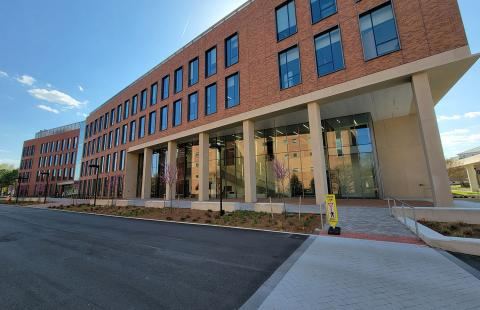
\includegraphics[width=\columnwidth]{Figures/cos_landscape.jpg}
\caption[The figure title goes here.]{The figure title goes here. Please describe the figure and figure legends here.}
\label{fig:logo_landscape}
\end{sidewaysfigure}
\chapter{Related Work}

Lorem ipsum dolor sit amet, consectetur adipiscing elit. In non molestie odio. Pellentesque volutpat, sem a viverra dictum, leo est scelerisque risus, ut convallis dui nulla a lacus. Proin mi magna, pharetra non ante sit amet, euismod lobortis odio. Donec gravida eu elit quis sagittis. Duis consequat, elit in fermentum rutrum, tellus dolor sodales ante, ac aliquam libero purus eu nisi. In aliquam nibh maximus varius blandit. Sed consequat libero faucibus vehicula gravida. Suspendisse vitae nisi ex. Quisque gravida risus ac dapibus blandit. Vestibulum mollis sollicitudin justo. Donec vel ipsum non ligula efficitur consequat. Morbi vulputate feugiat diam, rhoncus vehicula eros posuere vitae. Pellentesque sed egestas metus. Vestibulum libero elit, euismod quis vestibulum nec, vulputate at risus. In accumsan sem eu porta ultrices. Quisque sagittis massa felis, eget varius metus semper id. Vivamus tincidunt ipsum sem, sit amet eleifend diam tempor nec. Vivamus elementum, diam id lobortis mattis, nisi lacus.

\section{Section title}
Lorem ipsum dolor sit amet, consectetur adipiscing elit. In non molestie odio. Pellentesque volutpat, sem a viverra dictum, leo est scelerisque risus, ut convallis dui nulla a lacus. Proin mi magna, pharetra non ante sit amet, euismod lobortis odio. Donec gravida eu elit quis sagittis. Duis consequat, elit in fermentum rutrum, tellus dolor sodales ante, ac aliquam libero purus eu nisi. Donec gravida eu elit quis sagittis. Duis consequat, elit in fermentum rutrum, tellus dolor sodales ante, ac aliquam libero purus eu nisi.  

\section{Section title}
Lorem ipsum dolor sit amet, consectetur adipiscing elit. In non molestie odio. Pellentesque volutpat, sem a viverra dictum, leo est scelerisque risus, ut convallis dui nulla a lacus. Proin mi magna, pharetra non ante sit amet, euismod lobortis odio. Donec gravida eu elit quis sagittis. Duis consequat, elit in fermentum rutrum, tellus dolor sodales ante, ac aliquam libero purus eu nisi. 

\section{Section title}
Lorem ipsum dolor sit amet, consectetur adipiscing elit. In non molestie odio. Pellentesque volutpat, sem a viverra dictum, leo est scelerisque risus, ut convallis dui nulla a lacus. Proin mi magna, pharetra non ante sit amet, euismod lobortis odio. Donec gravida eu elit quis sagittis. Duis consequat, elit in fermentum rutrum, tellus dolor sodales ante, ac aliquam libero purus eu nisi. 

\section{Section title}
Lorem ipsum dolor sit amet, consectetur adipiscing elit. In non molestie odio. Pellentesque volutpat, sem a viverra dictum, leo est scelerisque risus, ut convallis dui nulla a lacus. Proin mi magna, pharetra non ante sit amet, euismod lobortis odio. Donec gravida eu elit quis sagittis. Duis consequat, elit in fermentum rutrum, tellus dolor sodales ante, ac aliquam libero purus eu nisi. 

\begin{table}[tbh]
%\caption[short title for list of tables - no period at end per EE 9/23]{long title for text}
\caption[The title of the table goes here. Duis consequat, elit in fermentum rutrum, tellus dolor sodales ante, ac aliquam libero purus eu nisi.]{The title of the table goes here. Duis consequat, elit in fermentum rutrum, tellus dolor sodales ante, ac aliquam libero purus eu nisi.}
\label{tab:table_example1}
\begin{center}
\begin{tabular}{lll}
      & Mean  & SD   \\ \hline
Row 1 & 21.13 & 2.98 \\ 
Row 2 & 13.40 & 1.75 \\ 
Row 3 & 33.20 & 5.53 \\ \hline
\end{tabular}
% \addtabletext{nomenclature for the TSs refers to the numbered species in the table.}
\end{center}
\end{table}

\section{Section Title}
Duis consequat, elit in fermentum rutrum, tellus dolor sodales ante, ac aliquam libero purus eu nisi. In aliquam nibh maximus varius blandit. Sed consequat libero faucibus vehicula gravida. Suspendisse vitae nisi ex. Quisque gravida risus ac dapibus blandit. Vestibulum mollis sollicitudin justo. Donec vel ipsum non ligula efficitur consequat.


\section{Section Title}
Morbi vulputate feugiat diam, rhoncus vehicula eros posuere vitae. Pellentesque sed egestas metus. Vestibulum libero elit, euismod quis vestibulum nec, vulputate at risus. In accumsan sem eu porta ultrices. Quisque sagittis massa felis, eget varius metus semper id. Vivamus tincidunt ipsum sem, sit amet eleifend diam tempor nec. Vivamus elementum, diam id lobortis mattis, nisi lacus. Morbi vulputate feugiat diam, rhoncus vehicula eros posuere vitae. Pellentesque sed egestas metus. Vestibulum libero elit, euismod quis vestibulum nec, vulputate at risus. In accumsan sem eu porta ultrices. Quisque sagittis massa felis, eget varius metus semper id. Vivamus tincidunt ipsum sem, sit amet eleifend diam tempor nec. Vivamus elementum, diam id lobortis mattis, nisi lacus. Morbi vulputate feugiat diam, rhoncus vehicula eros posuere vitae. Pellentesque sed egestas metus. Vestibulum libero elit, euismod quis vestibulum nec, vulputate at risus. In accumsan sem eu porta ultrices. Quisque sagittis massa felis, eget varius metus semper id. Vivamus tincidunt ipsum sem, sit amet eleifend diam tempor nec. Vivamus elementum, diam id lobortis mattis, nisi lacus. Morbi vulputate feugiat diam, rhoncus vehicula eros posuere vitae. 

\chapter{Chapter Title - This is a very long chapter name which needs to be wrapped onto the next line }

Lorem ipsum dolor sit amet, consectetur adipiscing elit. In non molestie odio. Pellentesque volutpat, sem a viverra dictum, leo est scelerisque risus, ut convallis dui nulla a lacus. Proin mi magna, pharetra non ante sit amet, euismod lobortis odio. Donec gravida eu elit quis sagittis. Duis consequat, elit in fermentum rutrum, tellus dolor sodales ante, ac aliquam libero purus eu nisi. In aliquam nibh maximus varius blandit. Sed consequat libero faucibus vehicula gravida. Suspendisse vitae nisi ex. Quisque gravida risus ac dapibus blandit. Vestibulum mollis sollicitudin justo. Donec vel ipsum non ligula efficitur consequat. Morbi vulputate feugiat diam, rhoncus vehicula eros posuere vitae. Pellentesque sed egestas metus. Vestibulum libero elit, euismod quis vestibulum nec, vulputate at risus. In accumsan sem eu porta ultrices. Quisque sagittis massa felis, eget varius metus semper id. Vivamus tincidunt ipsum sem, sit amet eleifend diam tempor nec. Vivamus elementum, diam id lobortis mattis, nisi lacus.

\begin{figure}[tbh]
  \centering
  %
\includegraphics{Figures/cos1.jpeg}
  %To set height width
  
\includegraphics[height=4cm]{Figures/cos1.jpeg}
  \caption[The figure title goes here.]{The figure title goes here. Please describe the figure and figure legends here.}
  \label{fig:cos1_1}
\end{figure}

Lorem ipsum dolor sit amet, consectetur adipiscing elit. In non molestie odio. Pellentesque volutpat, sem a viverra dictum, leo est scelerisque risus, ut convallis dui nulla a lacus. Proin mi magna, pharetra non ante sit amet, euismod lobortis odio. Donec gravida eu elit quis sagittis. Duis consequat, elit in fermentum rutrum, tellus dolor sodales ante, ac aliquam libero purus eu nisi. In aliquam nibh maximus varius blandit. Sed consequat libero faucibus vehicula gravida. Suspendisse vitae nisi ex. Quisque gravida risus ac dapibus blandit. Vestibulum mollis sollicitudin justo. Donec vel ipsum non ligula efficitur consequat. Morbi vulputate feugiat diam, rhoncus vehicula eros posuere vitae. Pellentesque sed egestas metus. Vestibulum libero elit, euismod quis vestibulum nec, vulputate at risus. In accumsan sem eu porta ultrices. Quisque sagittis massa felis, eget varius metus semper id. Vivamus tincidunt ipsum sem, sit amet eleifend diam tempor nec. Vivamus elementum, diam id lobortis mattis, nisi lacus.

\begin{figure}[tbh]
  \centering
  %
\includegraphics{Figures/cos1.jpeg}
  %To set height width
  
\includegraphics[height=4cm]{Figures/cos1.jpeg}
  \caption[The figure title goes here.]{The figure title goes here. Please describe the figure and figure legends here.}
  \label{fig:cos1_2}
\end{figure}

\begin{figure}[tbh]
  \centering
  %
\includegraphics{Figures/cos1.jpeg}
  %To set height width
  
\includegraphics[height=4cm]{Figures/cos1.jpeg}
  \caption[The figure title goes here.]{The figure title goes here. Please describe the figure and figure legends here.}
  \label{fig:cos1_3}
\end{figure}

Lorem ipsum dolor sit amet, consectetur adipiscing elit. In non molestie odio. Pellentesque volutpat, sem a viverra dictum, leo est scelerisque risus, ut convallis dui nulla a lacus. Proin mi magna, pharetra non ante sit amet, euismod lobortis odio. Donec gravida eu elit quis sagittis. Duis consequat, elit in fermentum rutrum, tellus dolor sodales ante, ac aliquam libero purus eu nisi. In aliquam nibh maximus varius blandit. Sed consequat libero faucibus vehicula gravida. Suspendisse vitae nisi ex. Quisque gravida risus ac dapibus blandit. Vestibulum mollis sollicitudin justo. Donec vel ipsum non ligula efficitur consequat. Morbi vulputate feugiat diam, rhoncus vehicula eros posuere vitae. Pellentesque sed egestas metus. Vestibulum libero elit, euismod quis vestibulum nec, vulputate at risus. In accumsan sem eu porta ultrices. Quisque sagittis massa felis, eget varius metus semper id. Vivamus tincidunt ipsum sem, sit amet eleifend diam tempor nec. Vivamus elementum, diam id lobortis mattis, nisi lacus.

\begin{figure}[tbh]
  \centering
  %
\includegraphics{Figures/cos1.jpeg}
  %To set height width
  
\includegraphics[height=4cm]{Figures/cos1.jpeg}
  \caption[The figure title goes here.]{The figure title goes here. Please describe the figure and figure legends here.}
  \label{fig:cos1_4}
\end{figure}

Lorem ipsum dolor sit amet, consectetur adipiscing elit. In non molestie odio. Pellentesque volutpat, sem a viverra dictum, leo est scelerisque risus, ut convallis dui nulla a lacus. Proin mi magna, pharetra non ante sit amet, euismod lobortis odio. Donec gravida eu elit quis sagittis. Duis consequat, elit in fermentum rutrum, tellus dolor sodales ante, ac aliquam libero purus eu nisi. In aliquam nibh maximus varius blandit. Sed consequat libero faucibus vehicula gravida. Suspendisse vitae nisi ex. Quisque gravida risus ac dapibus blandit. Vestibulum mollis sollicitudin justo. Donec vel ipsum non ligula efficitur consequat. Morbi vulputate feugiat diam, rhoncus vehicula eros posuere vitae. Pellentesque sed egestas metus. Vestibulum libero elit, euismod quis vestibulum nec, vulputate at risus. In accumsan sem eu porta ultrices. Quisque sagittis massa felis, eget varius metus semper id. Vivamus tincidunt ipsum sem, sit amet eleifend diam tempor nec. Vivamus elementum, diam id lobortis mattis, nisi lacus.

\begin{figure}[tbh]
  \centering
  %
\includegraphics{Figures/cos1.jpeg}
  %To set height width
  
\includegraphics[height=4cm]{Figures/cos1.jpeg}
  \caption[The figure title goes here.]{The figure title goes here. Please describe the figure and figure legends here.}
  \label{fig:cos1_5}
\end{figure}

Lorem ipsum dolor sit amet, consectetur adipiscing elit. In non molestie odio. Pellentesque volutpat, sem a viverra dictum, leo est scelerisque risus, ut convallis dui nulla a lacus. Proin mi magna, pharetra non ante sit amet, euismod lobortis odio. Donec gravida eu elit quis sagittis. 

\begin{table}[tbh]
%\caption[short title for list of tables - no period at end per EE 9/23]{long title for text}
\caption[The title of the table goes here.]{The title of the table goes here.}
\label{tab:table_example1_1}
\begin{center}
\begin{tabular}{lll}
      & Mean  & SD   \\ \hline
Row 1 & 21.13 & 2.98 \\ 
Row 2 & 13.40 & 1.75 \\ 
Row 3 & 33.20 & 5.53 \\ \hline
\end{tabular}
% \addtabletext{nomenclature for the TSs refers to the numbered species in the table.}
\end{center}
\end{table}

Eros posuere vitae. Pellentesque sed egestas metus. Vestibulum libero elit, euismod quis vestibulum nec, vulputate at risus. In accumsan sem eu porta ultrices. Quisque sagittis massa felis, eget varius metus semper id. Vivamus tincidunt ipsum sem, sit amet eleifend diam tempor nec. Vivamus elementum, diam id lobortis mattis, nisi lacus.

In aliquam nibh maximus varius blandit. Sed consequat libero faucibus vehicula gravida. Suspendisse vitae nisi ex. Quisque gravida risus ac dapibus blandit. Vestibulum mollis sollicitudin justo. Donec vel ipsum non ligula efficitur consequat. Morbi vulputate feugiat diam, rhoncus vehicula eros posuere vitae. Pellentesque sed egestas metus. Vestibulum libero elit, euismod quis vestibulum nec, vulputate at risus. 

\begin{figure}[tbh]
  \centering
  %
\includegraphics{Figures/cos1.jpeg}
  %To set height width
  
\includegraphics[height=4cm]{Figures/cos1.jpeg}
  \caption[The figure title goes here.]{The figure title goes here. Please describe the figure and figure legends here.}
  \label{fig:cos1_6}
\end{figure}

\section{Section Title}
Lorem ipsum dolor sit amet, consectetur adipiscing elit. In non molestie odio. Pellentesque volutpat, sem a viverra dictum, leo est scelerisque risus, ut convallis dui nulla a lacus. Proin mi magna, pharetra non ante sit amet, euismod lobortis odio. Donec gravida eu elit quis sagittis. Duis consequat, elit in fermentum rutrum, tellus dolor sodales ante, ac aliquam libero purus eu nisi. In aliquam nibh maximus varius blandit. Sed consequat libero faucibus vehicula gravida. Suspendisse vitae nisi ex. Quisque gravida risus ac dapibus blandit. Vestibulum mollis sollicitudin justo. Donec vel ipsum non ligula efficitur consequat. Morbi vulputate feugiat diam, rhoncus vehicula eros posuere vitae. Pellentesque sed egestas metus. Vestibulum libero elit, euismod quis vestibulum nec, vulputate at risus. In accumsan sem eu porta ultrices. Quisque sagittis massa felis, eget varius metus semper id. Vivamus tincidunt ipsum sem, sit amet eleifend diam tempor nec. Vivamus elementum, diam id lobortis mattis, nisi lacus. In accumsan sem eu porta ultrices. Quisque sagittis massa felis, eget varius metus semper id. Vivamus tincidunt ipsum sem, sit amet eleifend diam tempor nec. Vivamus elementum, diam id lobortis mattis, nisi lacus.
\begin{figure}[tbh]
  \centering
  %
\includegraphics{Figures/cos1.jpeg}
  %To set height width
  
\includegraphics[height=4cm]{Figures/cos1.jpeg}
  \caption[The figure title goes here.]{The figure title goes here. Please describe the figure and figure legends here.}
  \label{fig:cos1_7}
\end{figure}


Lorem ipsum dolor sit amet, consectetur adipiscing elit. In non molestie odio. Pellentesque volutpat, sem a viverra dictum, leo est scelerisque risus, ut convallis dui nulla a lacus. Proin mi magna, pharetra non ante sit amet, euismod lobortis odio. In accumsan sem eu porta ultrices. Quisque sagittis massa felis, eget varius metus semper id. Vivamus tincidunt ipsum sem, sit amet eleifend diam tempor nec. Vivamus elementum, diam id lobortis mattis, nisi lacus.

\begin{table}[tbh]
%\caption[short title for list of tables - no period at end per EE 9/23]{long title for text}
\caption[The title of the table goes here.]{The title of the table goes here.}
\label{tab:table_example1_2}
\begin{center}
\begin{tabular}{lll}
      & Mean  & SD   \\ \hline
Row 1 & 21.13 & 2.98 \\ 
Row 2 & 13.40 & 1.75 \\ 
Row 3 & 33.20 & 5.53 \\ \hline
\end{tabular}
% \addtabletext{nomenclature for the TSs refers to the numbered species in the table.}
\end{center}
\end{table}

In aliquam nibh maximus varius blandit. Sed consequat libero faucibus vehicula gravida. Suspendisse vitae nisi ex. Quisque gravida risus ac dapibus blandit. Vestibulum mollis sollicitudin justo. Donec vel ipsum non ligula efficitur consequat. Morbi vulputate feugiat diam, rhoncus vehicula eros posuere vitae. Pellentesque sed egestas metus. Vestibulum libero elit, euismod quis vestibulum nec, vulputate at risus. In accumsan sem eu porta ultrices. Quisque sagittis massa felis, eget varius metus semper id. Vivamus tincidunt ipsum sem, sit amet eleifend diam tempor nec. Vivamus elementum, diam id lobortis mattis, nisi lacus. Pellentesque sed egestas metus. Vestibulum libero elit, euismod quis vestibulum nec, vulputate at risus. In accumsan sem eu porta ultrices.

Donec gravida eu elit quis sagittis. Duis consequat, elit in fermentum rutrum, tellus dolor sodales ante, ac aliquam libero purus eu nisi. In aliquam nibh maximus varius blandit.

\begin{figure}[tbh]
  \centering
  %
\includegraphics{Figures/cos1.jpeg}
  %To set height width
  
\includegraphics[height=4cm]{Figures/cos1.jpeg}
  \caption[The figure title goes here.]{The figure title goes here. Please describe the figure and figure legends here.}
  \label{fig:cos1_8}
\end{figure}

Lorem ipsum dolor sit amet, consectetur adipiscing elit. In non molestie odio. Pellentesque volutpat, sem a viverra dictum, leo est scelerisque risus, ut convallis dui nulla a lacus. Proin mi magna, pharetra non ante sit amet, euismod lobortis odio. Donec gravida eu elit quis sagittis. Duis consequat, elit in fermentum rutrum, tellus dolor sodales ante, ac aliquam libero purus eu nisi. In aliquam nibh maximus varius blandit. Sed consequat libero faucibus vehicula gravida. Suspendisse vitae nisi ex. Quisque gravida risus ac dapibus blandit. Vestibulum mollis sollicitudin justo. Donec vel ipsum non ligula efficitur consequat. Morbi vulputate feugiat diam, rhoncus vehicula eros posuere vitae. Pellentesque sed egestas metus. Vestibulum libero elit, euismod quis vestibulum nec, vulputate at risus. In accumsan sem eu porta ultrices. Quisque sagittis massa felis, eget varius metus semper id. Vivamus tincidunt ipsum sem, sit amet eleifend diam tempor nec. Vivamus elementum, diam id lobortis mattis, nisi lacus. Pellentesque sed egestas metus. Vestibulum libero elit, euismod quis vestibulum nec, vulputate at risus.

\begin{figure}[tbh]
  \centering
  %
\includegraphics{Figures/cos1.jpeg}
  %To set height width
  
\includegraphics[height=4cm]{Figures/cos1.jpeg}
  \caption[The figure title goes here.]{The figure title goes here. Please describe the figure and figure legends here.}
  \label{fig:cos1_9}
\end{figure}


Lorem ipsum dolor sit amet, consectetur adipiscing elit. In non molestie odio. Pellentesque volutpat, sem a viverra dictum, leo est scelerisque risus, ut convallis dui nulla a lacus. Proin mi magna, pharetra non ante sit amet, euismod lobortis odio. Donec gravida eu elit quis sagittis. Duis consequat, elit in fermentum rutrum, tellus dolor sodales ante, ac aliquam libero purus eu nisi. In aliquam nibh maximus varius blandit. Sed consequat libero faucibus vehicula gravida. Suspendisse vitae nisi ex. Quisque gravida risus ac dapibus blandit. Vestibulum mollis sollicitudin justo. Donec vel ipsum non ligula efficitur consequat. Morbi vulputate feugiat diam, rhoncus vehicula eros posuere vitae. Pellentesque sed egestas metus. Vestibulum libero elit, euismod quis vestibulum nec, vulputate at risus. In accumsan sem eu porta ultrices. Quisque sagittis massa felis, eget varius metus semper id. Vivamus tincidunt ipsum sem, sit amet eleifend diam tempor nec. Vivamus elementum, diam id lobortis mattis, nisi lacus.

\begin{figure}[tbh]
  \centering
  %
\includegraphics{Figures/cos1.jpeg}
  %To set height width
  
\includegraphics[height=4cm]{Figures/cos1.jpeg}
  \caption[The figure title goes here.]{The figure title goes here. Please describe the figure and figure legends here.}
  \label{fig:cos1_10}
\end{figure}

\section{Section Title}
In aliquam nibh maximus varius blandit. Sed consequat libero faucibus vehicula gravida. Suspendisse vitae nisi ex. Quisque gravida risus ac dapibus blandit. Vestibulum mollis sollicitudin justo. Donec vel ipsum non ligula efficitur consequat. Morbi vulputate feugiat diam, rhoncus vehicula eros posuere vitae. Pellentesque sed egestas metus. Vestibulum libero elit, euismod quis vestibulum nec, vulputate at risus. In accumsan sem eu porta ultrices. Quisque sagittis massa felis, eget varius metus semper id. Vivamus tincidunt ipsum sem, sit amet eleifend diam tempor nec. Vivamus elementum, diam id lobortis mattis, nisi lacus. Pellentesque sed egestas metus. Vestibulum libero elit, euismod quis vestibulum nec, vulputate at risus. In accumsan sem eu porta ultrices.


\begin{figure}[tbh]
  \centering
  %
\includegraphics{Figures/cos1.jpeg}
  %To set height width
  
\includegraphics[height=4cm]{Figures/cos1.jpeg}
  \caption[The figure title goes here.]{The figure title goes here. Please describe the figure and figure legends here.}
  \label{fig:cos1_11}
\end{figure}

Lorem ipsum dolor sit amet, consectetur adipiscing elit. In non molestie odio. Pellentesque volutpat, sem a viverra dictum, leo est scelerisque risus, ut convallis dui nulla a lacus. Proin mi magna, pharetra non ante sit amet, euismod lobortis odio. Donec gravida eu elit quis sagittis. Duis consequat, elit in fermentum rutrum, tellus dolor sodales ante, ac aliquam libero purus eu nisi. In aliquam nibh maximus varius blandit. Sed consequat libero faucibus vehicula gravida. Suspendisse vitae nisi ex. Quisque gravida risus ac dapibus blandit. Vestibulum mollis sollicitudin justo. Donec vel ipsum non ligula efficitur consequat. Morbi vulputate feugiat diam, rhoncus vehicula eros posuere vitae. Pellentesque sed egestas metus. Vestibulum libero elit, euismod quis vestibulum nec, vulputate at risus. In accumsan sem eu porta ultrices. 


\begin{table}[tbh]
%\caption[short title for list of tables - no period at end per EE 9/23]{long title for text}
\caption[The title of the table goes here.]{The title of the table goes here.}
\label{tab:table_example1_3}
\begin{center}
\begin{tabular}{lll}
      & Mean  & SD   \\ \hline
Row 1 & 21.13 & 2.98 \\ 
Row 2 & 13.40 & 1.75 \\ 
Row 3 & 33.20 & 5.53 \\ \hline
\end{tabular}
% \addtabletext{nomenclature for the TSs refers to the numbered species in the table.}
\end{center}
\end{table}

In aliquam nibh maximus varius blandit. Sed consequat libero faucibus vehicula gravida. Suspendisse vitae nisi ex. Quisque gravida risus ac dapibus blandit. Vestibulum mollis sollicitudin justo. Donec vel ipsum non ligula efficitur consequat. Morbi vulputate feugiat diam, rhoncus vehicula eros posuere vitae. Pellentesque sed egestas metus. Vestibulum libero elit, euismod quis vestibulum nec, vulputate at risus. In accumsan sem eu porta ultrices. Quisque sagittis massa felis, eget varius metus semper id. Vivamus tincidunt ipsum sem, sit amet eleifend diam tempor nec. Vivamus elementum, diam id lobortis mattis, nisi lacus.

Quisque sagittis massa felis, eget varius metus semper id. Vivamus tincidunt ipsum sem, sit amet eleifend diam tempor nec. Vivamus elementum, diam id lobortis mattis, nisi lacus. Lorem ipsum dolor sit amet, consectetur adipiscing elit. In non molestie odio. Pellentesque volutpat, sem a viverra dictum, leo est scelerisque risus, ut convallis dui nulla a lacus. Proin mi magna, pharetra non ante sit amet, euismod lobortis odio. Donec gravida eu elit quis sagittis. Duis consequat, elit in fermentum rutrum, tellus dolor sodales ante, ac aliquam libero purus eu nisi. In aliquam nibh maximus varius blandit. Sed consequat libero faucibus vehicula gravida. Suspendisse vitae nisi ex. Quisque gravida risus ac dapibus blandit. Vestibulum mollis sollicitudin justo. Donec vel ipsum non ligula efficitur consequat. Morbi vulputate feugiat diam, rhoncus vehicula eros posuere vitae. Pellentesque sed egestas metus. Vestibulum libero elit, euismod quis vestibulum nec, vulputate at risus. 

\begin{figure}[tbh]
  \centering
  %
\includegraphics{Figures/cos1.jpeg}
  %To set height width
  
\includegraphics[height=4cm]{Figures/cos1.jpeg}
  \caption[The figure title goes here.]{The figure title goes here. Please describe the figure and figure legends here.}
  \label{fig:cos1_12}
\end{figure}


\begin{figure}[tbh]
  \centering
  %
\includegraphics{Figures/cos1.jpeg}
  %To set height width
  
\includegraphics[height=4cm]{Figures/cos1.jpeg}
  \caption[The figure title goes here.]{The figure title goes here. Please describe the figure and figure legends here.}
  \label{fig:cos1_13}
\end{figure}

Lorem ipsum dolor sit amet, consectetur adipiscing elit. In non molestie odio. Pellentesque volutpat, sem a viverra dictum, leo est scelerisque risus, ut convallis dui nulla a lacus. Proin mi magna, pharetra non ante sit amet, euismod lobortis odio. Donec gravida eu elit quis sagittis. Duis consequat, elit in fermentum rutrum, tellus dolor sodales ante, ac aliquam libero purus eu nisi. In aliquam nibh maximus varius blandit. Sed consequat libero faucibus vehicula gravida. Suspendisse vitae nisi ex. Quisque gravida risus ac dapibus blandit. Vestibulum mollis sollicitudin justo. Donec vel ipsum non ligula efficitur consequat. Morbi vulputate feugiat diam, rhoncus vehicula eros posuere vitae. Pellentesque sed egestas metus. Vestibulum libero elit, euismod quis vestibulum nec, vulputate at risus. In accumsan sem eu porta ultrices. Quisque sagittis massa felis, eget varius metus semper id. Vivamus tincidunt ipsum sem, sit amet eleifend diam tempor nec. Vivamus elementum, diam id lobortis mattis, nisi lacus.

\begin{table}[tbh]
%\caption[short title for list of tables - no period at end per EE 9/23]{long title for text}
\caption[The title of the table goes here.]{The title of the table goes here.}
\label{tab:table_example1_4}
\begin{center}
\begin{tabular}{lll}
      & Mean  & SD   \\ \hline
Row 1 & 21.13 & 2.98 \\ 
Row 2 & 13.40 & 1.75 \\ 
Row 3 & 33.20 & 5.53 \\ \hline
\end{tabular}
% \addtabletext{nomenclature for the TSs refers to the numbered species in the table.}
\end{center}
\end{table}


\section{Section Title}
Lorem ipsum dolor sit amet, consectetur adipiscing elit. In non molestie odio. Pellentesque volutpat, sem a viverra dictum, leo est scelerisque risus, ut convallis dui nulla a lacus. Proin mi magna, pharetra non ante sit amet, euismod lobortis odio. Donec gravida eu elit quis sagittis. Duis consequat, elit in fermentum rutrum, tellus dolor sodales ante, ac aliquam libero purus eu nisi. In aliquam nibh maximus varius blandit. Sed consequat libero faucibus vehicula gravida. Suspendisse vitae nisi ex. Quisque gravida risus ac dapibus blandit. Vestibulum mollis sollicitudin justo. Donec vel ipsum non ligula efficitur consequat. Morbi vulputate feugiat diam, rhoncus vehicula eros posuere vitae. Pellentesque sed egestas metus. Vestibulum libero elit, euismod quis vestibulum nec, vulputate at risus. 

\begin{figure}[tbh]
  \centering
  %
\includegraphics{Figures/cos1.jpeg}
  %To set height width
  
\includegraphics[height=4cm]{Figures/cos1.jpeg}
  \caption[The figure title goes here.]{The figure title goes here. Please describe the figure and figure legends here.}
  \label{fig:cos1_14}
\end{figure}

Suspendisse vitae nisi ex. Quisque gravida risus ac dapibus blandit. Vestibulum mollis sollicitudin justo. Donec vel ipsum non ligula efficitur consequat. Morbi vulputate feugiat diam, rhoncus vehicula eros posuere vitae. Pellentesque sed egestas metus. Vestibulum libero elit, euismod quis vestibulum nec, vulputate at risus. In accumsan sem eu porta ultrices. Quisque sagittis massa felis, eget varius metus semper id. Vivamus tincidunt ipsum sem, sit amet eleifend diam tempor nec. Vivamus elementum, diam id lobortis mattis, nisi lacus. In accumsan sem eu porta ultrices. Quisque sagittis massa felis, eget varius metus semper id. In accumsan sem eu porta ultrices. Quisque sagittis massa felis, eget varius metus semper id. 

\begin{figure}[tbh]
  \centering
  %
\includegraphics{Figures/cos1.jpeg}
  %To set height width
  
\includegraphics[height=4cm]{Figures/cos1.jpeg}
  \caption[The figure title goes here.]{The figure title goes here. Please describe the figure and figure legends here.}
  \label{fig:cos1_15}
\end{figure}

Suspendisse vitae nisi ex. Quisque gravida risus ac dapibus blandit. Vestibulum mollis sollicitudin justo. Donec vel ipsum non ligula efficitur consequat. Morbi vulputate feugiat diam, rhoncus vehicula eros posuere vitae. Pellentesque sed egestas metus. Vestibulum libero elit, euismod quis vestibulum nec, vulputate at risus. In accumsan sem eu porta ultrices. Quisque sagittis massa felis, eget varius metus semper id. Vivamus tincidunt ipsum sem, sit amet eleifend diam tempor nec. Vivamus elementum, diam id lobortis mattis, nisi lacus. 


\begin{figure}[tbh]
  \centering
  %
\includegraphics{Figures/cos1.jpeg}
  %To set height width
  
\includegraphics[height=4cm]{Figures/cos1.jpeg}
  \caption[The figure title goes here.]{The figure title goes here. Please describe the figure and figure legends here.}
  \label{fig:cos1_16}
\end{figure}


\begin{figure}[tbh]
  \centering
  %
\includegraphics{Figures/cos1.jpeg}
  %To set height width
  
\includegraphics[height=4cm]{Figures/cos1.jpeg}
  \caption[The figure title goes here.]{The figure title goes here. Please describe the figure and figure legends here.}
  \label{fig:cos1_17}
\end{figure}

Suspendisse vitae nisi ex. Quisque gravida risus ac dapibus blandit. Vestibulum mollis sollicitudin justo. Donec vel ipsum non ligula efficitur consequat. Morbi vulputate feugiat diam, rhoncus vehicula eros posuere vitae. Pellentesque sed egestas metus. Vestibulum libero elit, euismod quis vestibulum nec, vulputate at risus. In accumsan sem eu porta ultrices. Quisque sagittis massa felis, eget varius metus semper id. 



\begin{figure}[tbh]
  \centering
  %
\includegraphics{Figures/cos1.jpeg}
  %To set height width
  
\includegraphics[height=4cm]{Figures/cos1.jpeg}
  \caption[The figure title goes here.]{The figure title goes here. Please describe the figure and figure legends here.}
  \label{fig:cos1_18}
\end{figure}


\begin{figure}[tbh]
  \centering
  %
\includegraphics{Figures/cos1.jpeg}
  %To set height width
  
\includegraphics[height=4cm]{Figures/cos1.jpeg}
  \caption[The figure title goes here.]{The figure title goes here. Please describe the figure and figure legends here.}
  \label{fig:cos1_19}
\end{figure}

Suspendisse vitae nisi ex. Quisque gravida risus ac dapibus blandit. Vestibulum mollis sollicitudin justo. Donec vel ipsum non ligula efficitur consequat. Morbi vulputate feugiat diam, rhoncus vehicula eros posuere vitae. Pellentesque sed egestas metus. Vestibulum libero elit, euismod quis vestibulum nec, vulputate at risus. In accumsan sem eu porta ultrices. Quisque sagittis massa felis, eget varius metus semper id. Vivamus tincidunt ipsum sem, sit amet eleifend diam tempor nec. Vivamus elementum, diam id lobortis mattis, nisi lacus. Suspendisse vitae nisi ex. Quisque gravida risus ac dapibus blandit. Vestibulum mollis sollicitudin justo. Donec vel ipsum non ligula efficitur consequat. Morbi vulputate feugiat diam, rhoncus vehicula eros posuere vitae. Pellentesque sed egestas metus. Vestibulum libero elit, euismod quis vestibulum nec, vulputate at risus. In accumsan sem eu porta ultrices. Quisque sagittis massa felis, eget varius metus semper id. Vivamus tincidunt ipsum sem, sit amet eleifend diam tempor nec. Vivamus elementum, diam id lobortis mattis, nisi lacus. Suspendisse vitae nisi ex. Quisque gravida risus ac dapibus blandit. Vestibulum mollis sollicitudin justo. Donec vel ipsum non ligula efficitur consequat. Morbi vulputate feugiat diam, rhoncus vehicula eros posuere vitae. Pellentesque sed egestas metus. Vestibulum libero elit, euismod quis vestibulum nec, vulputate at risus. In accumsan sem eu porta ultrices. Quisque sagittis massa felis, eget varius metus semper id. Vivamus tincidunt ipsum sem, sit amet eleifend diam tempor nec. Vivamus elementum, diam id lobortis mattis, nisi lacus.




\begin{figure}[tbh]
  \centering
  %
\includegraphics{Figures/cos1.jpeg}
  %To set height width
  
\includegraphics[height=4cm]{Figures/cos1.jpeg}
  \caption[The figure title goes here.]{The figure title goes here. Please describe the figure and figure legends here.}
  \label{fig:cos1_20}
\end{figure}


\begin{figure}[tbh]
  \centering
  %
\includegraphics{Figures/cos1.jpeg}
  %To set height width
  
\includegraphics[height=4cm]{Figures/cos1.jpeg}
  \caption[The figure title goes here.]{The figure title goes here. Please describe the figure and figure legends here.}
  \label{fig:cos1_21}
\end{figure}


Suspendisse vitae nisi ex. Quisque gravida risus ac dapibus blandit. Vestibulum mollis sollicitudin justo. Donec vel ipsum non ligula efficitur consequat. Morbi vulputate feugiat diam, rhoncus vehicula eros posuere vitae. Pellentesque sed egestas metus. Vestibulum libero elit, euismod quis vestibulum nec, vulputate at risus. In accumsan sem eu porta ultrices. Quisque sagittis massa felis, eget varius metus semper id. Vivamus tincidunt ipsum sem, sit amet eleifend diam tempor nec. Vivamus elementum, diam id lobortis mattis, nisi lacus.

\begin{figure}[tbh]
  \centering
  %\includegraphics{Figures/cos1.jpeg}
  %To set height width
  \includegraphics[height=4cm]{Figures/cos1.jpeg}
  \caption[The figure title goes here.]{The figure title goes here. Please describe the figure and figure legends here.}
  \label{fig:cos1_22}
\end{figure}

\section{Section Title}
Lorem ipsum dolor sit amet, consectetur adipiscing elit. In non molestie odio. Pellentesque volutpat, sem a viverra dictum, leo est scelerisque risus, ut convallis dui nulla a lacus. Proin mi magna, pharetra non ante sit amet, euismod lobortis odio. Donec gravida eu elit quis sagittis. Duis consequat, elit in fermentum rutrum, tellus dolor sodales ante, ac aliquam libero purus eu nisi. 

\begin{figure}[tbh]
  \centering
  %\includegraphics{Figures/cos1.jpeg}
  %To set height width
  \includegraphics[height=4cm]{Figures/cos1.jpeg}
  \caption[The figure title goes here.]{The figure title goes here. Please describe the figure and figure legends here.}
  \label{fig:cos1_23}
\end{figure}


\section{Section Title}
In aliquam nibh maximus varius blandit. Sed consequat libero faucibus vehicula gravida. Suspendisse vitae nisi ex. Quisque gravida risus ac dapibus blandit. Vestibulum mollis sollicitudin justo. Donec vel ipsum non ligula efficitur consequat. Morbi vulputate feugiat diam, rhoncus vehicula eros posuere vitae. Pellentesque sed egestas metus. Vestibulum libero elit, euismod quis vestibulum nec, vulputate at risus. In accumsan sem eu porta ultrices. Quisque sagittis massa felis, eget varius metus semper id. Vivamus tincidunt ipsum sem, sit amet eleifend diam tempor nec. Vivamus elementum, diam id lobortis mattis, nisi lacus.


\begin{table}
%\caption[short title for list of tables]{long title for text}
\caption[The title of the table goes here.]{The title of the table goes here. Duis consequat, elit in fermentum rutrum, tellus dolor sodales ante, ac aliquam libero purus eu nisi.}
\label{tab:table_example2}
\begin{center}
\begin{tabular}{lll}
      & Mean  & SD   \\ \hline
Row 1 & 21.13 & 2.98 \\ 
Row 2 & 13.40 & 1.75 \\ 
Row 3 & 33.20 & 5.53 \\ \hline
\end{tabular}
\end{center}
\end{table}

In aliquam nibh maximus varius blandit. Sed consequat libero faucibus vehicula gravida. Suspendisse vitae nisi ex. Quisque gravida risus ac dapibus blandit. Vestibulum mollis sollicitudin justo. Donec vel ipsum non ligula efficitur consequat. Morbi vulputate feugiat diam, rhoncus vehicula eros posuere vitae. Pellentesque sed egestas metus. Vestibulum libero elit, euismod quis vestibulum nec, vulputate at risus. In accumsan sem eu porta ultrices. Quisque sagittis massa felis, eget varius metus semper id. Vivamus tincidunt ipsum sem, sit amet eleifend diam tempor nec. Vivamus elementum, diam id lobortis mattis, nisi lacus. Quisque sagittis massa felis, eget varius metus semper id. Vivamus tincidunt ipsum sem, sit amet eleifend diam tempor nec. Vivamus elementum, diam id lobortis mattis, nisi lacus. Quisque sagittis massa felis, eget varius metus semper id. Vivamus tincidunt ipsum sem, sit amet eleifend diam tempor nec. Vivamus elementum, diam id lobortis mattis, nisi lacus.




\chapter{Chapter Title}

Lorem ipsum dolor sit amet, consectetur adipiscing elit. In non molestie odio. Pellentesque volutpat, sem a viverra dictum, leo est scelerisque risus, ut convallis dui nulla a lacus. Proin mi magna, pharetra non ante sit amet, euismod lobortis odio. Donec gravida eu elit quis sagittis. Duis consequat, elit in fermentum rutrum, tellus dolor sodales ante, ac aliquam libero purus eu nisi. In aliquam nibh maximus varius blandit. Sed consequat libero faucibus vehicula gravida. Suspendisse vitae nisi ex. Quisque gravida risus ac dapibus blandit. Vestibulum mollis sollicitudin justo. Donec vel ipsum non ligula efficitur consequat. Morbi vulputate feugiat diam, rhoncus vehicula eros posuere vitae. Pellentesque sed egestas metus. Vestibulum libero elit, euismod quis vestibulum nec, vulputate at risus. In accumsan sem eu porta ultrices. Quisque sagittis massa felis, eget varius metus semper id. Vivamus tincidunt ipsum sem, sit amet eleifend diam tempor nec. Vivamus elementum, diam id lobortis mattis, nisi lacus. Quisque sagittis massa felis, eget varius metus semper id. Vivamus tincidunt ipsum sem, sit amet eleifend diam tempor nec. Vivamus elementum, diam id lobortis mattis, nisi lacus.


\section{Section Title}
Lorem ipsum dolor sit amet, consectetur adipiscing elit. In non molestie odio. Pellentesque volutpat, sem a viverra dictum, leo est scelerisque risus, ut convallis dui nulla a lacus. Proin mi magna, pharetra non ante sit amet, euismod lobortis odio. Donec gravida eu elit quis sagittis. Duis consequat, elit in fermentum rutrum, tellus dolor sodales ante, ac aliquam libero purus eu nisi. 


\section{Section Title}
In aliquam nibh maximus varius blandit. Sed consequat libero faucibus vehicula gravida. Suspendisse vitae nisi ex. Quisque gravida risus ac dapibus blandit. Vestibulum mollis sollicitudin justo. Donec vel ipsum non ligula efficitur consequat. Morbi vulputate feugiat diam, rhoncus vehicula eros posuere vitae. Pellentesque sed egestas metus. Vestibulum libero elit, euismod quis vestibulum nec, vulputate at risus. In accumsan sem eu porta ultrices. Quisque sagittis massa felis, eget varius metus semper id. Vivamus tincidunt ipsum sem, sit amet eleifend diam tempor nec. Vivamus elementum, diam id lobortis mattis, nisi lacus.

\section{Section Title}
In aliquam nibh maximus varius blandit. Sed consequat libero faucibus vehicula gravida. Suspendisse vitae nisi ex. Quisque gravida risus ac dapibus blandit. Vestibulum mollis sollicitudin justo. Donec vel ipsum non ligula efficitur consequat. Morbi vulputate feugiat diam, rhoncus vehicula eros posuere vitae. Pellentesque sed egestas metus. Vestibulum libero elit, euismod quis vestibulum nec, vulputate at risus. In accumsan sem eu porta ultrices. Quisque sagittis massa felis, eget varius metus semper id. Vivamus tincidunt ipsum sem, sit amet eleifend diam tempor nec. Vivamus elementum, diam id lobortis mattis, nisi lacus.


\section{Section Title}
In aliquam nibh maximus varius blandit. Sed consequat libero faucibus vehicula gravida. Suspendisse vitae nisi ex. Quisque gravida risus ac dapibus blandit. Vestibulum mollis sollicitudin justo. Donec vel ipsum non ligula efficitur consequat. Morbi vulputate feugiat diam, rhoncus vehicula eros posuere vitae. Pellentesque sed egestas metus. Vestibulum libero elit, euismod quis vestibulum nec, vulputate at risus. In accumsan sem eu porta ultrices. Quisque sagittis massa felis, eget varius metus semper id. Vivamus tincidunt ipsum sem, sit amet eleifend diam tempor nec. Vivamus elementum, diam id lobortis mattis, nisi lacus. In aliquam nibh maximus varius blandit. Sed consequat libero faucibus vehicula gravida. Suspendisse vitae nisi ex. Quisque gravida risus ac dapibus blandit. Vestibulum mollis sollicitudin justo. Donec vel ipsum non ligula efficitur consequat. Morbi vulputate feugiat diam, rhoncus vehicula eros posuere vitae. Pellentesque sed egestas metus. Vestibulum libero elit, euismod quis vestibulum nec, vulputate at risus. In accumsan sem eu porta ultrices. Quisque sagittis massa felis, eget varius metus semper id. Vivamus tincidunt ipsum sem, sit amet eleifend diam tempor nec. Vivamus elementum, diam id lobortis mattis, nisi lacus.

\begin{table}[tbh]
\caption[The title of the table goes here.]{The title of the table goes here.}
\label{tab:table_example1_5}
\begin{center}
\begin{tabular}{lll}
      & Mean  & SD   \\ \hline
Row 1 & 21.13 & 2.98 \\ 
Row 2 & 13.40 & 1.75 \\ 
Row 3 & 33.20 & 5.53 \\ \hline
\end{tabular}
\end{center}
\end{table}

In aliquam nibh maximus varius blandit. Sed consequat libero faucibus vehicula gravida. Suspendisse vitae nisi ex. Quisque gravida risus ac dapibus blandit. Vestibulum mollis sollicitudin justo. Donec vel ipsum non ligula efficitur consequat. Morbi vulputate feugiat diam, rhoncus vehicula eros posuere vitae. Pellentesque sed egestas metus. Vestibulum libero elit, euismod quis vestibulum nec, vulputate at risus. In accumsan sem eu porta ultrices. Quisque sagittis massa felis, eget varius metus semper id. Vivamus tincidunt ipsum sem, sit amet eleifend diam tempor nec. Vivamus elementum, diam id lobortis mattis, nisi lacus. In aliquam nibh maximus varius blandit. Sed consequat libero faucibus vehicula gravida. Suspendisse vitae nisi ex. Quisque gravida risus ac dapibus blandit. Vestibulum mollis sollicitudin justo. Donec vel ipsum non ligula efficitur consequat. Morbi vulputate feugiat diam, rhoncus vehicula eros posuere vitae. Pellentesque sed egestas metus. Vestibulum libero elit, euismod quis vestibulum nec, vulputate at risus. In accumsan sem eu porta ultrices. Quisque sagittis massa felis, eget varius metus semper id. Vivamus tincidunt ipsum sem, sit amet eleifend diam tempor nec. Vivamus elementum, diam id lobortis mattis, nisi lacus.

Quisque sagittis massa felis, eget varius metus semper id. Vivamus tincidunt ipsum sem, sit amet eleifend diam tempor nec. Vivamus elementum, diam id lobortis mattis, nisi lacus. Quisque sagittis massa felis, eget varius metus semper id. Vivamus tincidunt ipsum sem, sit amet eleifend diam tempor nec. Vivamus elementum, diam id lobortis mattis, nisi lacus. Quisque sagittis massa felis, eget varius metus semper id. Vivamus tincidunt ipsum sem, sit amet eleifend diam tempor nec. Vivamus elementum, diam id lobortis mattis, nisi lacus. Quisque sagittis massa felis, eget varius metus semper id. Vivamus tincidunt ipsum sem, sit amet eleifend diam tempor nec. Vivamus elementum, diam id lobortis mattis, nisi lacus. Quisque sagittis massa felis, eget varius metus semper id. Vivamus tincidunt ipsum sem, sit amet eleifend diam tempor nec. Vivamus elementum, diam id lobortis mattis, nisi lacus. 
 

\chapter{Chapter Title}

Lorem ipsum dolor sit amet, consectetur adipiscing elit. In non molestie odio. Pellentesque volutpat, sem a viverra dictum, leo est scelerisque risus, ut convallis dui nulla a lacus. Proin mi magna, pharetra non ante sit amet, euismod lobortis odio. Donec gravida eu elit quis sagittis. Duis consequat, elit in fermentum rutrum, tellus dolor sodales ante, ac aliquam libero purus eu nisi. In aliquam nibh maximus varius blandit. Sed consequat libero faucibus vehicula gravida. Suspendisse vitae nisi ex. Quisque gravida risus ac dapibus blandit. Vestibulum mollis sollicitudin justo. Donec vel ipsum non ligula efficitur consequat. Morbi vulputate feugiat diam, rhoncus vehicula eros posuere vitae. Pellentesque sed egestas metus. Vestibulum libero elit, euismod quis vestibulum nec, vulputate at risus. In accumsan sem eu porta ultrices. Quisque sagittis massa felis, eget varius metus semper id. Vivamus tincidunt ipsum sem, sit amet eleifend diam tempor nec. Vivamus elementum, diam id lobortis mattis, nisi lacus.


\begin{table}[tbh]
\caption[The title of the table goes here.]{The title of the table goes here.}
\label{tab:table_example1_6}
\begin{center}
\begin{tabular}{lll}
      & Mean  & SD   \\ \hline
Row 1 & 21.13 & 2.98 \\ 
Row 2 & 13.40 & 1.75 \\ 
Row 3 & 33.20 & 5.53 \\ \hline
\end{tabular}
\end{center}
\end{table}

In aliquam nibh maximus varius blandit. Sed consequat libero faucibus vehicula gravida. Suspendisse vitae nisi ex. Quisque gravida risus ac dapibus blandit. Vestibulum mollis sollicitudin justo. Donec vel ipsum non ligula efficitur consequat. Morbi vulputate feugiat diam, rhoncus vehicula eros posuere vitae. Pellentesque sed egestas metus. Vestibulum libero elit, euismod quis vestibulum nec, vulputate at risus. In accumsan sem eu porta ultrices. Quisque sagittis massa felis, eget varius metus semper id. Vivamus tincidunt ipsum sem, sit amet eleifend diam tempor nec. Vivamus elementum, diam id lobortis mattis, nisi lacus.

\begin{table}[tbh]
\caption[The title of the table goes here.]{The title of the table goes here.}
\label{tab:table_example1_7}
\begin{center}
\begin{tabular}{lll}
      & Mean  & SD   \\ \hline
Row 1 & 21.13 & 2.98 \\ 
Row 2 & 13.40 & 1.75 \\ 
Row 3 & 33.20 & 5.53 \\ \hline
\end{tabular}
\end{center}
\end{table}

In aliquam nibh maximus varius blandit. Sed consequat libero faucibus vehicula gravida. Suspendisse vitae nisi ex. Quisque gravida risus ac dapibus blandit. Vestibulum mollis sollicitudin justo. Donec vel ipsum non ligula efficitur consequat. Morbi vulputate feugiat diam, rhoncus vehicula eros posuere vitae. Pellentesque sed egestas metus. Vestibulum libero elit, euismod quis vestibulum nec, vulputate at risus. In accumsan sem eu porta ultrices. Quisque sagittis massa felis, eget varius metus semper id. Vivamus tincidunt ipsum sem, sit amet eleifend diam tempor nec. 

\begin{table}[tbh]
\caption[The title of the table goes here.]{The title of the table goes here.}
\label{tab:table_example1_8}
\begin{center}
\begin{tabular}{lll}
      & Mean  & SD   \\ \hline
Row 1 & 21.13 & 2.98 \\ 
Row 2 & 13.40 & 1.75 \\ 
Row 3 & 33.20 & 5.53 \\ \hline
\end{tabular}
\end{center}
\end{table}

\section{Section Title}
In aliquam nibh maximus varius blandit. Sed consequat libero faucibus vehicula gravida. Suspendisse vitae nisi ex. Quisque gravida risus ac dapibus blandit. Vestibulum mollis sollicitudin justo. Donec vel ipsum non ligula efficitur consequat. Morbi vulputate feugiat diam, rhoncus vehicula eros posuere vitae. Pellentesque sed egestas metus. Vestibulum libero elit, euismod quis vestibulum nec, vulputate at risus. In accumsan sem eu porta ultrices. Quisque sagittis massa felis, eget varius metus semper id. Vivamus tincidunt ipsum sem, sit amet eleifend diam tempor nec. Vivamus elementum, diam id lobortis mattis, nisi lacus.

\begin{table}[tbh]
\caption[The title of the table goes here.]{The title of the table goes here.}
\label{tab:table_example1_9}
\begin{center}
\begin{tabular}{lll}
      & Mean  & SD   \\ \hline
Row 1 & 21.13 & 2.98 \\ 
Row 2 & 13.40 & 1.75 \\ 
Row 3 & 33.20 & 5.53 \\ \hline
\end{tabular}
\end{center}
\end{table}

\begin{table}[tbh]
\caption[The title of the table goes here.]{The title of the table goes here.}
\label{tab:table_example1_10}
\begin{center}
\begin{tabular}{lll}
      & Mean  & SD   \\ \hline
Row 1 & 21.13 & 2.98 \\ 
Row 2 & 13.40 & 1.75 \\ 
Row 3 & 33.20 & 5.53 \\ \hline
\end{tabular}
\end{center}
\end{table}


In aliquam nibh maximus varius blandit. Sed consequat libero faucibus vehicula gravida. Suspendisse vitae nisi ex. Quisque gravida risus ac dapibus blandit. Vestibulum mollis sollicitudin justo. Donec vel ipsum non ligula efficitur consequat. Morbi vulputate feugiat diam, rhoncus vehicula eros posuere vitae. Pellentesque sed egestas metus. Vestibulum libero elit, euismod quis vestibulum nec, vulputate at risus. In accumsan sem eu porta ultrices. Quisque sagittis massa felis, eget varius metus semper id. Vivamus tincidunt ipsum sem, sit amet eleifend diam tempor nec. Vivamus elementum, diam id lobortis mattis, nisi lacus.


\begin{table}[tbh]
\caption[The title of the table goes here.]{The title of the table goes here.}
\label{tab:table_example1_11}
\begin{center}
\begin{tabular}{lll}
      & Mean  & SD   \\ \hline
Row 1 & 21.13 & 2.98 \\ 
Row 2 & 13.40 & 1.75 \\ 
Row 3 & 33.20 & 5.53 \\ \hline
\end{tabular}
\end{center}
\end{table}


In aliquam nibh maximus varius blandit. Sed consequat libero faucibus vehicula gravida. Suspendisse vitae nisi ex. Quisque gravida risus ac dapibus blandit. Vestibulum mollis sollicitudin justo. Donec vel ipsum non ligula efficitur consequat. Morbi vulputate feugiat diam, rhoncus vehicula eros posuere vitae. Pellentesque sed egestas metus. Vestibulum libero elit, euismod quis vestibulum nec, vulputate at risus. In accumsan sem eu porta ultrices. Quisque sagittis massa felis, eget varius metus semper id. Vivamus tincidunt ipsum sem, sit amet eleifend diam tempor nec. Vivamus elementum, diam id lobortis mattis, nisi lacus.

\begin{table}[tbh]
\caption[The title of the table goes here.]{The title of the table goes here.}
\label{tab:table_example1_12}
\begin{center}
\begin{tabular}{lll}
      & Mean  & SD   \\ \hline
Row 1 & 21.13 & 2.98 \\ 
Row 2 & 13.40 & 1.75 \\ 
Row 3 & 33.20 & 5.53 \\ \hline
\end{tabular}
\end{center}
\end{table}


In aliquam nibh maximus varius blandit. Sed consequat libero faucibus vehicula gravida. Suspendisse vitae nisi ex. Quisque gravida risus ac dapibus blandit. Vestibulum mollis sollicitudin justo. Donec vel ipsum non ligula efficitur consequat. Morbi vulputate feugiat diam, rhoncus vehicula eros posuere vitae. Pellentesque sed egestas metus. Vestibulum libero elit, euismod quis vestibulum nec, vulputate at risus. In accumsan sem eu porta ultrices. Quisque sagittis massa felis, eget varius metus semper id. Vivamus tincidunt ipsum sem, sit amet eleifend diam tempor nec. Vivamus elementum, diam id lobortis mattis, nisi lacus. 
In aliquam nibh maximus varius blandit. Sed consequat libero faucibus vehicula gravida. Suspendisse vitae nisi ex. Quisque gravida risus ac dapibus blandit. Vestibulum mollis sollicitudin justo. Donec vel ipsum non ligula efficitur consequat. Morbi vulputate feugiat diam, rhoncus vehicula eros posuere vitae. Pellentesque sed egestas metus. Vestibulum libero elit, euismod quis vestibulum nec, vulputate at risus. In accumsan sem eu porta ultrices. Quisque sagittis massa felis, eget varius metus semper id. Vivamus tincidunt ipsum sem, sit amet eleifend diam tempor nec. Vivamus elementum, diam id lobortis mattis, nisi lacus. 
In aliquam nibh maximus varius blandit. Sed consequat libero faucibus vehicula gravida. Suspendisse vitae nisi ex. Quisque gravida risus ac dapibus blandit. Vestibulum mollis sollicitudin justo. Donec vel ipsum non ligula efficitur consequat. Morbi vulputate feugiat diam, rhoncus vehicula eros posuere vitae. Pellentesque sed egestas metus. Vestibulum libero elit, euismod quis vestibulum nec, vulputate at risus. In accumsan sem eu porta ultrices. Quisque sagittis massa felis, eget varius metus semper id. Vivamus tincidunt ipsum sem, sit amet eleifend diam tempor nec. Vivamus elementum, diam id lobortis mattis, nisi lacus.




\begin{table}[tbh]
\caption[The title of the table goes here.]{The title of the table goes here.}
\label{tab:table_example1_13}
\begin{center}
\begin{tabular}{lll}
      & Mean  & SD   \\ \hline
Row 1 & 21.13 & 2.98 \\ 
Row 2 & 13.40 & 1.75 \\ 
Row 3 & 33.20 & 5.53 \\ \hline
\end{tabular}
\end{center}
\end{table}

\begin{table}[tbh]
\caption[The title of the table goes here.]{The title of the table goes here.}
\label{tab:table_example1_14}
\begin{center}
\begin{tabular}{lll}
      & Mean  & SD   \\ \hline
Row 1 & 21.13 & 2.98 \\ 
Row 2 & 13.40 & 1.75 \\ 
Row 3 & 33.20 & 5.53 \\ \hline
\end{tabular}
\end{center}
\end{table}


In aliquam nibh maximus varius blandit. Sed consequat libero faucibus vehicula gravida. Suspendisse vitae nisi ex. Quisque gravida risus ac dapibus blandit. Vestibulum mollis sollicitudin justo. Donec vel ipsum non ligula efficitur consequat. Morbi vulputate feugiat diam, rhoncus vehicula eros posuere vitae. Pellentesque sed egestas metus. Vestibulum libero elit, euismod quis vestibulum nec, vulputate at risus. In accumsan sem eu porta ultrices. Quisque sagittis massa felis, eget varius metus semper id. Vivamus tincidunt ipsum sem, sit amet eleifend diam tempor nec. Vivamus elementum, diam id lobortis mattis, nisi lacus. 
In aliquam nibh maximus varius blandit. Sed consequat libero faucibus vehicula gravida. Suspendisse vitae nisi ex. Quisque gravida risus ac dapibus blandit. Vestibulum mollis sollicitudin justo. Donec vel ipsum non ligula efficitur consequat. Morbi vulputate feugiat diam, rhoncus vehicula eros posuere vitae. Pellentesque sed egestas metus. Vestibulum libero elit, euismod quis vestibulum nec, vulputate at risus. In accumsan sem eu porta ultrices. Quisque sagittis massa felis, eget varius metus semper id. Vivamus tincidunt ipsum sem, sit amet eleifend diam tempor nec. Vivamus elementum, diam id lobortis mattis, nisi lacus.



\begin{table}[tbh]
\caption[The title of the table goes here.]{The title of the table goes here.}
\label{tab:table_example1_15}
\begin{center}
\begin{tabular}{lll}
      & Mean  & SD   \\ \hline
Row 1 & 21.13 & 2.98 \\ 
Row 2 & 13.40 & 1.75 \\ 
Row 3 & 33.20 & 5.53 \\ \hline
\end{tabular}
\end{center}
\end{table}


In aliquam nibh maximus varius blandit. Sed consequat libero faucibus vehicula gravida. Suspendisse vitae nisi ex. Quisque gravida risus ac dapibus blandit. Vestibulum mollis sollicitudin justo. Donec vel ipsum non ligula efficitur consequat. Morbi vulputate feugiat diam, rhoncus vehicula eros posuere vitae. Pellentesque sed egestas metus. Vestibulum libero elit, euismod quis vestibulum nec, vulputate at risus. In accumsan sem eu porta ultrices. Quisque sagittis massa felis, eget varius metus semper id. Vivamus tincidunt ipsum sem, sit amet eleifend diam tempor nec. Vivamus elementum, diam id lobortis mattis, nisi lacus.


\section{Section Title}
Lorem ipsum dolor sit amet, consectetur adipiscing elit. In non molestie odio. Pellentesque volutpat, sem a viverra dictum, leo est scelerisque risus, ut convallis dui nulla a lacus. Proin mi magna, pharetra non ante sit amet, euismod lobortis odio. Donec gravida eu elit quis sagittis. Duis consequat, elit in fermentum rutrum, tellus dolor sodales ante, ac aliquam libero purus eu nisi. 


\begin{table}[tbh]
\caption[The title of the table goes here.]{The title of the table goes here.}
\label{tab:table_example1_16}
\begin{center}
\begin{tabular}{lll}
      & Mean  & SD   \\ \hline
Row 1 & 21.13 & 2.98 \\ 
Row 2 & 13.40 & 1.75 \\ 
Row 3 & 33.20 & 5.53 \\ \hline
\end{tabular}
\end{center}
\end{table}


In aliquam nibh maximus varius blandit. Sed consequat libero faucibus vehicula gravida. Suspendisse vitae nisi ex. Quisque gravida risus ac dapibus blandit. Vestibulum mollis sollicitudin justo. Donec vel ipsum non ligula efficitur consequat. Morbi vulputate feugiat diam, rhoncus vehicula eros posuere vitae. Pellentesque sed egestas metus. Vestibulum libero elit, euismod quis vestibulum nec, vulputate at risus. In accumsan sem eu porta ultrices. Quisque sagittis massa felis, eget varius metus semper id. Vivamus tincidunt ipsum sem, sit amet eleifend diam tempor nec. Vivamus elementum, diam id lobortis mattis, nisi lacus. 
In aliquam nibh maximus varius blandit. Sed consequat libero faucibus vehicula gravida. Suspendisse vitae nisi ex. Quisque gravida risus ac dapibus blandit. Vestibulum mollis sollicitudin justo. Donec vel ipsum non ligula efficitur consequat. Morbi vulputate feugiat diam, rhoncus vehicula eros posuere vitae. Pellentesque sed egestas metus. Vestibulum libero elit, euismod quis vestibulum nec, vulputate at risus. In accumsan sem eu porta ultrices. Quisque sagittis massa felis, eget varius metus semper id. Vivamus tincidunt ipsum sem, sit amet eleifend diam tempor nec. Vivamus elementum, diam id lobortis mattis, nisi lacus.



\begin{table}[tbh]
\caption[The title of the table goes here.]{The title of the table goes here.}
\label{tab:table_example1_17}
\begin{center}
\begin{tabular}{lll}
      & Mean  & SD   \\ \hline
Row 1 & 21.13 & 2.98 \\ 
Row 2 & 13.40 & 1.75 \\ 
Row 3 & 33.20 & 5.53 \\ \hline
\end{tabular}
\end{center}
\end{table}

\section{Section Title}
In aliquam nibh maximus varius blandit. Sed consequat libero faucibus vehicula gravida. Suspendisse vitae nisi ex. Quisque gravida risus ac dapibus blandit. Vestibulum mollis sollicitudin justo. Donec vel ipsum non ligula efficitur consequat. Morbi vulputate feugiat diam, rhoncus vehicula eros posuere vitae. Pellentesque sed egestas metus. Vestibulum libero elit, euismod quis vestibulum nec, vulputate at risus. In accumsan sem eu porta ultrices. Quisque sagittis massa felis, eget varius metus semper id. Vivamus tincidunt ipsum sem, sit amet eleifend diam tempor nec. Vivamus elementum, diam id lobortis mattis, nisi lacus.


\begin{table}[tbh]
\caption[The title of the table goes here.]{The title of the table goes here.}
\label{tab:table_example1_18}
\begin{center}
\begin{tabular}{lll}
      & Mean  & SD   \\ \hline
Row 1 & 21.13 & 2.98 \\ 
Row 2 & 13.40 & 1.75 \\ 
Row 3 & 33.20 & 5.53 \\ \hline
\end{tabular}
\end{center}
\end{table}


In aliquam nibh maximus varius blandit. Sed consequat libero faucibus vehicula gravida. Suspendisse vitae nisi ex. Quisque gravida risus ac dapibus blandit. Vestibulum mollis sollicitudin justo. Donec vel ipsum non ligula efficitur consequat. Morbi vulputate feugiat diam, rhoncus vehicula eros posuere vitae. Pellentesque sed egestas metus. Vestibulum libero elit, euismod quis vestibulum nec, vulputate at risus. In accumsan sem eu porta ultrices. Quisque sagittis massa felis, eget varius metus semper id. Vivamus tincidunt ipsum sem, sit amet eleifend diam tempor nec. Vivamus elementum, diam id lobortis mattis, nisi lacus.


\begin{table}[tbh]
\caption[The title of the table goes here.]{The title of the table goes here.}
\label{tab:table_example1_19}
\begin{center}
\begin{tabular}{lll}
      & Mean  & SD   \\ \hline
Row 1 & 21.13 & 2.98 \\ 
Row 2 & 13.40 & 1.75 \\ 
Row 3 & 33.20 & 5.53 \\ \hline
\end{tabular}
\end{center}
\end{table}

\section{Section Title}
In aliquam nibh maximus varius blandit. Sed consequat libero faucibus vehicula gravida. Suspendisse vitae nisi ex. Quisque gravida risus ac dapibus blandit. Vestibulum mollis sollicitudin justo. Donec vel ipsum non ligula efficitur consequat. Morbi vulputate feugiat diam, rhoncus vehicula eros posuere vitae. Pellentesque sed egestas metus. Vestibulum libero elit, euismod quis vestibulum nec, vulputate at risus. In accumsan sem eu porta ultrices. Quisque sagittis massa felis, eget varius metus semper id. 


\begin{table}[tbh]
\caption[The title of the table goes here.]{The title of the table goes here.}
\label{tab:table_example1_20}
\begin{center}
\begin{tabular}{lll}
      & Mean  & SD   \\ \hline
Row 1 & 21.13 & 2.98 \\ 
Row 2 & 13.40 & 1.75 \\ 
Row 3 & 33.20 & 5.53 \\ \hline
\end{tabular}
\end{center}
\end{table}


In aliquam nibh maximus varius blandit. Sed consequat libero faucibus vehicula gravida. Suspendisse vitae nisi ex. Quisque gravida risus ac dapibus blandit. Vestibulum mollis sollicitudin justo. Donec vel ipsum non ligula efficitur consequat. Morbi vulputate feugiat diam, rhoncus vehicula eros posuere vitae. Pellentesque sed egestas metus. Vestibulum libero elit, euismod quis vestibulum nec, vulputate at risus. In accumsan sem eu porta ultrices. Quisque sagittis massa felis, eget varius metus semper id. Vivamus tincidunt ipsum sem, sit amet eleifend diam tempor nec. Vivamus elementum, diam id lobortis mattis, nisi lacus. 
In aliquam nibh maximus varius blandit. Sed consequat libero faucibus vehicula gravida. Suspendisse vitae nisi ex. Quisque gravida risus ac dapibus blandit. Vestibulum mollis sollicitudin justo. Donec vel ipsum non ligula efficitur consequat. Morbi vulputate feugiat diam, rhoncus vehicula eros posuere vitae. Pellentesque sed egestas metus. Vestibulum libero elit, euismod quis vestibulum nec, vulputate at risus. In accumsan sem eu porta ultrices. Quisque sagittis massa felis, eget varius metus semper id. Vivamus tincidunt ipsum sem, sit amet eleifend diam tempor nec. Vivamus elementum, diam id lobortis mattis, nisi lacus. 
In aliquam nibh maximus varius blandit. Sed consequat libero faucibus vehicula gravida. Suspendisse vitae nisi ex. Quisque gravida risus ac dapibus blandit. Vestibulum mollis sollicitudin justo. Donec vel ipsum non ligula efficitur consequat. Morbi vulputate feugiat diam, rhoncus vehicula eros posuere vitae. Pellentesque sed egestas metus. Vestibulum libero elit, euismod quis vestibulum nec, vulputate at risus. In accumsan sem eu porta ultrices. Quisque sagittis massa felis, eget varius metus semper id. Vivamus tincidunt ipsum sem, sit amet eleifend diam tempor nec. Vivamus elementum, diam id lobortis mattis, nisi lacus.



\section{Section Title}
In aliquam nibh maximus varius blandit. Sed consequat libero faucibus vehicula gravida. Suspendisse vitae nisi ex. Quisque gravida risus ac dapibus blandit. Vestibulum mollis sollicitudin justo. Donec vel ipsum non ligula efficitur consequat. Morbi vulputate feugiat diam, rhoncus vehicula eros posuere vitae. Pellentesque sed egestas metus. Vestibulum libero elit, euismod quis vestibulum nec, vulputate at risus. In accumsan sem eu porta ultrices. Quisque sagittis massa felis, eget varius metus semper id. Vivamus tincidunt ipsum sem, sit amet eleifend diam tempor nec. Vivamus elementum, diam id lobortis mattis, nisi lacus.



\begin{table}[tbh]
\caption[The title of the table goes here.]{The title of the table goes here.}
\label{tab:table_example1_21}
\begin{center}
\begin{tabular}{lll}
      & Mean  & SD   \\ \hline
Row 1 & 21.13 & 2.98 \\ 
Row 2 & 13.40 & 1.75 \\ 
Row 3 & 33.20 & 5.53 \\ \hline
\end{tabular}
\end{center}
\end{table}

\chapter{Future Work}
Lorem ipsum dolor sit amet, consectetur adipiscing elit. In non molestie odio. Pellentesque volutpat, sem a viverra dictum, leo est scelerisque risus, ut convallis dui nulla a lacus. Proin mi magna, pharetra non ante sit amet, euismod lobortis odio. Donec gravida eu elit quis sagittis. Duis consequat, elit in fermentum rutrum, tellus dolor sodales ante, ac aliquam libero purus eu nisi. In aliquam nibh maximus varius blandit. Sed consequat libero faucibus vehicula gravida. Suspendisse vitae nisi ex. Quisque gravida risus ac dapibus blandit. Vestibulum mollis sollicitudin justo. Donec vel ipsum non ligula efficitur consequat. Morbi vulputate feugiat diam, rhoncus vehicula eros posuere vitae. Pellentesque sed egestas metus. Vestibulum libero elit, euismod quis vestibulum nec, vulputate at risus. In accumsan sem eu porta ultrices. Quisque sagittis massa felis, eget varius metus semper id. Vivamus tincidunt ipsum sem, sit amet eleifend diam tempor nec. Vivamus elementum, diam id lobortis mattis, nisi lacus.

Lorem ipsum dolor sit amet, consectetur adipiscing elit. Pellentesque ac mauris luctus, laoreet mauris non, maximus justo. Nam semper laoreet orci a rhoncus. Pellentesque sed pellentesque purus. Vivamus et dapibus elit, id dapibus justo. Maecenas magna ipsum, rutrum a nisl ac, porta convallis nulla. Pellentesque ornare tempor ipsum, eu dictum mi ultrices vitae. Quisque enim lacus, posuere eget mollis in, ornare a eros. Aliquam laoreet nulla sit amet facilisis laoreet. Vivamus non est et ante luctus dignissim convallis eget massa. Suspendisse eu tortor a nibh consequat dictum. Nam semper laoreet orci a rhoncus. Pellentesque sed pellentesque purus. Vivamus et dapibus elit, id dapibus justo. Maecenas magna ipsum, rutrum a nisl ac, porta convallis nulla.

Vestibulum vitae quam vulputate, facilisis lorem nec, venenatis massa. Duis id odio pulvinar, semper est nec, placerat nisl. Aenean eget dui libero. Phasellus scelerisque convallis molestie. Sed sem quam, pharetra ut massa nec, viverra vestibulum odio. Morbi eu sem quis metus tempus eleifend quis non felis. Nullam ornare nulla eu dapibus ullamcorper. Mauris convallis risus id turpis semper pulvinar. Interdum et malesuada fames ac ante ipsum primis in faucibus. Nulla volutpat velit a dignissim facilisis. Mauris non eros eget est faucibus laoreet sit amet ut urna. Cras id condimentum magna. Sed sit amet dolor iaculis purus sodales vulputate id nec nunc. Sed ultrices justo vel orci rhoncus, eu tempor nunc convallis. Proin pretium sodales sem, quis porta sem feugiat eget.

Cras in convallis felis, ullamcorper volutpat nisi. Nunc sit amet consequat risus. Morbi urna dolor, scelerisque non risus nec, venenatis lobortis nunc. Mauris elementum porta nunc eu suscipit. Pellentesque porta dolor ligula, sit amet porta turpis pharetra sed. Vivamus malesuada augue tellus. Mauris pharetra neque ut velit pulvinar, non tempor nulla convallis. Integer et lorem turpis. Cras commodo ex lectus. Vestibulum ante ipsum primis in faucibus orci luctus et ultrices posuere cubilia curae; Vivamus suscipit nibh vitae nisl interdum, vel euismod arcu laoreet. Mauris id elit magna.

Quisque scelerisque molestie justo id dignissim. Morbi vel urna orci. Ut condimentum nisi purus, vitae finibus orci ultricies ultricies. Proin dolor neque, semper sit amet massa vitae, iaculis viverra magna. Proin leo sem, sodales ac nunc at, scelerisque imperdiet eros. Morbi velit arcu, auctor ut rutrum quis, pretium eu arcu. Curabitur semper mauris nisl, sit amet ullamcorper orci aliquet id. Sed euismod venenatis laoreet. Etiam accumsan tincidunt pharetra. Lorem ipsum dolor sit amet, consectetur adipiscing elit. Aenean pharetra euismod pellentesque.
\chapter{Conclusion}
Lorem ipsum dolor sit amet, consectetur adipiscing elit. In non molestie odio. Pellentesque volutpat, sem a viverra dictum, leo est scelerisque risus, ut convallis dui nulla a lacus. Proin mi magna, pharetra non ante sit amet, euismod lobortis odio. Donec gravida eu elit quis sagittis. Duis consequat, elit in fermentum rutrum, tellus dolor sodales ante, ac aliquam libero purus eu nisi. In aliquam nibh maximus varius blandit. Sed consequat libero faucibus vehicula gravida. Suspendisse vitae nisi ex. Quisque gravida risus ac dapibus blandit. Vestibulum mollis sollicitudin justo. Donec vel ipsum non ligula efficitur consequat. Morbi vulputate feugiat diam, rhoncus vehicula eros posuere vitae. Pellentesque sed egestas metus. Vestibulum libero elit, euismod quis vestibulum nec, vulputate at risus. In accumsan sem eu porta ultrices. Quisque sagittis massa felis, eget varius metus semper id. Vivamus tincidunt ipsum sem, sit amet eleifend diam tempor nec. Vivamus elementum, diam id lobortis mattis, nisi lacus.

Lorem ipsum dolor sit amet, consectetur adipiscing elit. Pellentesque ac mauris luctus, laoreet mauris non, maximus justo. Nam semper laoreet orci a rhoncus. Pellentesque sed pellentesque purus. Vivamus et dapibus elit, id dapibus justo. Maecenas magna ipsum, rutrum a nisl ac, porta convallis nulla. Pellentesque ornare tempor ipsum, eu dictum mi ultrices vitae. Quisque enim lacus, posuere eget mollis in, ornare a eros. Aliquam laoreet nulla sit amet facilisis laoreet. Vivamus non est et ante luctus dignissim convallis eget massa.

Vestibulum vitae quam vulputate, facilisis lorem nec, venenatis massa. Duis id odio pulvinar, semper est nec, placerat nisl. Aenean eget dui libero. Phasellus scelerisque convallis molestie. Sed sem quam, pharetra ut massa nec, viverra vestibulum odio. Morbi eu sem quis metus tempus eleifend quis non felis. Nullam ornare nulla eu dapibus ullamcorper. Mauris convallis risus id turpis semper pulvinar. Interdum et malesuada fames ac ante ipsum primis in faucibus. Nulla volutpat velit a dignissim facilisis. Mauris non eros eget est faucibus laoreet sit amet ut urna. Cras id condimentum magna. Sed sit amet dolor iaculis purus sodales vulputate id nec nunc. Sed ultrices justo vel orci rhoncus, eu tempor nunc convallis. Proin pretium sodales sem, quis porta sem feugiat eget.

Cras in convallis felis, ullamcorper volutpat nisi. Nunc sit amet consequat risus. Morbi urna dolor, scelerisque non risus nec, venenatis lobortis nunc. Mauris elementum porta nunc eu suscipit. Pellentesque porta dolor ligula, sit amet porta turpis pharetra sed. Vivamus malesuada augue tellus. Mauris pharetra neque ut velit pulvinar, non tempor nulla convallis. Integer et lorem turpis. Cras commodo ex lectus. Vestibulum ante ipsum primis in faucibus orci luctus et ultrices posuere cubilia curae; Vivamus suscipit nibh vitae nisl interdum, vel euismod arcu laoreet. Mauris id elit magna.

Quisque scelerisque molestie justo id dignissim. Morbi vel urna orci. Ut condimentum nisi purus, vitae finibus orci ultricies ultricies. Proin dolor neque, semper sit amet massa vitae, iaculis viverra magna. Proin leo sem, sodales ac nunc at, scelerisque imperdiet eros. Morbi velit arcu, auctor ut rutrum quis, pretium eu arcu. Curabitur semper mauris nisl, sit amet ullamcorper orci aliquet id. Sed euismod venenatis laoreet. Etiam accumsan tincidunt pharetra. Lorem ipsum dolor sit amet, consectetur adipiscing elit. Aenean pharetra euismod pellentesque.

\cleardoublepage

%%%%% REFERENCES %%%%% 
\addtocontents{toc}{\vspace*{12pt}} % gap between last chapter and references in the table of contents
\printbibliography[heading=bibintoc, title={REFERENCES}]

%%%%% APPENDICES %%%%% 
%% Comment the line below if you do not have any appendices
%%%%% If Appendices Needed %%%%%


\achapter{The Title of the Appendix A}

Lorem ipsum dolor sit amet, consectetur adipiscing elit. In non molestie odio. Pellentesque volutpat, sem a viverra dictum, leo est scelerisque risus, ut convallis dui nulla a lacus. 

\achapter{The Title of the Appendix B}

Lorem ipsum dolor sit amet, consectetur adipiscing elit. In non molestie odio. Pellentesque volutpat, sem a viverra dictum, leo est scelerisque risus, ut convallis dui nulla a lacus. 

\achapter{The Title of the Appendix C}

Lorem ipsum dolor sit amet, consectetur adipiscing elit. In non molestie odio. Pellentesque volutpat, sem a viverra dictum, leo est scelerisque risus, ut convallis dui nulla a lacus. 

\newpage


%%%%% VITA - max 1 page %%%%% 
% Vita goes here, this must be limited to one page
\vita{
\noindent \uppercase{\textbf{Education}} \\
% Include year(s), position, university 
% Include year(s), degree, major, university
\indent 2019-2022, Education history goes here. \\
\indent 2018-2019, Education history goes here.
\vspace{0.85cm} \\
\noindent \uppercase{\textbf{Professional Experience}} \\
% Include year(s), position, employee
\indent 2020-2022, Professional history goes here. \\
\indent 2018-2020, Professional history goes here.
\vspace{0.85cm}\\
\noindent \uppercase{\textbf{Conference Presentations}} 
% Include name, conference, presentation title, dates
\indent \begin{enumerate}[noitemsep,partopsep=0pt,topsep=0pt,parsep=0pt]
\item Presentation history goes here.
\item Presentation history goes here. 
\end{enumerate}
\vspace{0.85cm} 
\noindent \uppercase{\textbf{Publications}}
% Include authors, title, journal, vol, pages, year
\indent \begin{enumerate}[noitemsep,partopsep=0pt,topsep=0pt,parsep=0pt]
\item Publication history goes here.
\item Publication history goes here.
\end{enumerate}
\vspace{0.85cm} 
}

\vitapage


\end{document}
